% This template is borrowed from the Reed College LaTeX thesis template. Most of the work
% for the document class was done by Sam Noble (SN), as well as this
% template. Later comments etc. by Ben Salzberg (BTS). Additional
% restructuring and APA support by Jess Youngberg (JY).
% Your comments and suggestions are more than welcome; please email
% them to cus@reed.edu
%
% See http://web.reed.edu/cis/help/latex.html for help. There are a
% great bunch of help pages there, with notes on
% getting started, bibtex, etc. Go there and read it if you're not
% already familiar with LaTeX.
%
% Any line that starts with a percent symbol is a comment.
% They won't show up in the document, and are useful for notes
% to yourself and explaining commands.
% Commenting also removes a line from the document;
% very handy for troubleshooting problems. -BTS

% As far as I know, this follows the requirements laid out in
% the 2002-2003 Senior Handbook. Ask a librarian to check the
% document before binding. -SN

%%
%% Preamble
%%
% \documentclass{<something>} must begin each LaTeX document
\documentclass[12pt,twoside]{deuthesis}
% Packages are extensions to the basic LaTeX functions. Whatever you
% want to typeset, there is probably a package out there for it.
% Chemistry (chemtex), screenplays, you name it.
% Check out CTAN to see: http://www.ctan.org/
%%
\usepackage{graphicx,latexsym}
\usepackage{amsmath}
\usepackage{amssymb,amsthm}
\usepackage{longtable,booktabs,setspace}
\usepackage{chemarr} %% Useful for one reaction arrow, useless if you're not a chem major
\usepackage[hyphens]{url}
% Added by CII
\usepackage{hyperref}
\usepackage{lmodern}
\usepackage{float}
\floatplacement{figure}{H}
% End of CII addition
\usepackage{rotating}

% Next line commented out by CII
%%% \usepackage{natbib}
% Comment out the natbib line above and uncomment the following two lines to use the new
% biblatex-chicago style, for Chicago A. Also make some changes at the end where the
% bibliography is included.
%\usepackage{biblatex-chicago}
%\bibliography{thesis}


% Added by CII (Thanks, Hadley!)
% Use ref for internal links
\renewcommand{\hyperref}[2][???]{\autoref{#1}}
\def\chapterautorefname{Chapter}
\def\sectionautorefname{Section}
\def\subsectionautorefname{Subsection}
% End of CII addition

% Added by CII
\usepackage{caption}
\captionsetup{width=5in}
% End of CII addition

% \usepackage{times} % other fonts are available like times, bookman, charter, palatino

% Syntax highlighting #22
  \usepackage{color}
  \usepackage{fancyvrb}
  \newcommand{\VerbBar}{|}
  \newcommand{\VERB}{\Verb[commandchars=\\\{\}]}
  \DefineVerbatimEnvironment{Highlighting}{Verbatim}{commandchars=\\\{\}}
  % Add ',fontsize=\small' for more characters per line
  \usepackage{framed}
  \definecolor{shadecolor}{RGB}{248,248,248}
  \newenvironment{Shaded}{\begin{snugshade}}{\end{snugshade}}
  \newcommand{\AlertTok}[1]{\textcolor[rgb]{0.94,0.16,0.16}{#1}}
  \newcommand{\AnnotationTok}[1]{\textcolor[rgb]{0.56,0.35,0.01}{\textbf{\textit{#1}}}}
  \newcommand{\AttributeTok}[1]{\textcolor[rgb]{0.77,0.63,0.00}{#1}}
  \newcommand{\BaseNTok}[1]{\textcolor[rgb]{0.00,0.00,0.81}{#1}}
  \newcommand{\BuiltInTok}[1]{#1}
  \newcommand{\CharTok}[1]{\textcolor[rgb]{0.31,0.60,0.02}{#1}}
  \newcommand{\CommentTok}[1]{\textcolor[rgb]{0.56,0.35,0.01}{\textit{#1}}}
  \newcommand{\CommentVarTok}[1]{\textcolor[rgb]{0.56,0.35,0.01}{\textbf{\textit{#1}}}}
  \newcommand{\ConstantTok}[1]{\textcolor[rgb]{0.00,0.00,0.00}{#1}}
  \newcommand{\ControlFlowTok}[1]{\textcolor[rgb]{0.13,0.29,0.53}{\textbf{#1}}}
  \newcommand{\DataTypeTok}[1]{\textcolor[rgb]{0.13,0.29,0.53}{#1}}
  \newcommand{\DecValTok}[1]{\textcolor[rgb]{0.00,0.00,0.81}{#1}}
  \newcommand{\DocumentationTok}[1]{\textcolor[rgb]{0.56,0.35,0.01}{\textbf{\textit{#1}}}}
  \newcommand{\ErrorTok}[1]{\textcolor[rgb]{0.64,0.00,0.00}{\textbf{#1}}}
  \newcommand{\ExtensionTok}[1]{#1}
  \newcommand{\FloatTok}[1]{\textcolor[rgb]{0.00,0.00,0.81}{#1}}
  \newcommand{\FunctionTok}[1]{\textcolor[rgb]{0.00,0.00,0.00}{#1}}
  \newcommand{\ImportTok}[1]{#1}
  \newcommand{\InformationTok}[1]{\textcolor[rgb]{0.56,0.35,0.01}{\textbf{\textit{#1}}}}
  \newcommand{\KeywordTok}[1]{\textcolor[rgb]{0.13,0.29,0.53}{\textbf{#1}}}
  \newcommand{\NormalTok}[1]{#1}
  \newcommand{\OperatorTok}[1]{\textcolor[rgb]{0.81,0.36,0.00}{\textbf{#1}}}
  \newcommand{\OtherTok}[1]{\textcolor[rgb]{0.56,0.35,0.01}{#1}}
  \newcommand{\PreprocessorTok}[1]{\textcolor[rgb]{0.56,0.35,0.01}{\textit{#1}}}
  \newcommand{\RegionMarkerTok}[1]{#1}
  \newcommand{\SpecialCharTok}[1]{\textcolor[rgb]{0.00,0.00,0.00}{#1}}
  \newcommand{\SpecialStringTok}[1]{\textcolor[rgb]{0.31,0.60,0.02}{#1}}
  \newcommand{\StringTok}[1]{\textcolor[rgb]{0.31,0.60,0.02}{#1}}
  \newcommand{\VariableTok}[1]{\textcolor[rgb]{0.00,0.00,0.00}{#1}}
  \newcommand{\VerbatimStringTok}[1]{\textcolor[rgb]{0.31,0.60,0.02}{#1}}
  \newcommand{\WarningTok}[1]{\textcolor[rgb]{0.56,0.35,0.01}{\textbf{\textit{#1}}}}

% To pass between YAML and LaTeX the dollar signs are added by CII
\title{MAKİNE ÖĞRENMESİ YAKLAŞIMLARININ KARPAL TÜNEL SENDROMU CİDDİYET SINIFLAMASINDA KULLANILMASI}
%\author{Alper ENGİNAtadeniz SAYARCem GÖRENER} %Tek yazar için
\author{Alper ENGİN \\ Atadeniz SAYAR \\ Cem GÖRENER} %Çok yazar için
% The month and year that you submit your FINAL draft TO THE LIBRARY (May or December)
\date{Ocak 2022}
\division{İSTATİSTİK BÖLÜMÜ}
\advisor{Dr.~Engin YILDIZTEPE}
\institution{FEN FAKÜLTESİ}
\degree{Bitirme Projesi Raporu}
%If you have two advisors for some reason, you can use the following
% Uncommented out by CII
% End of CII addition

%%% Remember to use the correct department!
\department{İstatistik Bölümü}
% if you're writing a thesis in an interdisciplinary major,
% uncomment the line below and change the text as appropriate.
% check the Senior Handbook if unsure.
%\thedivisionof{The Established Interdisciplinary Committee for}
% if you want the approval page to say "Approved for the Committee",
% uncomment the next line
%\approvedforthe{Committee}

% Added by CII
%%% Copied from knitr
%% maxwidth is the original width if it's less than linewidth
%% otherwise use linewidth (to make sure the graphics do not exceed the margin)
\makeatletter
\def\maxwidth{ %
  \ifdim\Gin@nat@width>\linewidth
    \linewidth
  \else
    \Gin@nat@width
  \fi
}
\makeatother

\renewcommand{\contentsname}{Table of Contents}
% End of CII addition

\setlength{\parskip}{0pt}

% Added by CII

\providecommand{\tightlist}{%
  \setlength{\itemsep}{0pt}\setlength{\parskip}{0pt}}

\Acknowledgements{
Tüm çalışma süresince yönlendiriciliği, katkıları ve yardımları ile yanımızda olan danışmanımız Dr.~Engin YILDIZTEPE 'ye ve böyle bir çalışmayı yapmamız için bize fırsat tanıyan Dokuz Eylül Üniversitesi Fen Fakültesi İstatistik Bölümüne teşekkür ederiz.\\
\strut \\
\strut \\
Alper ENGİN\\
Atadeniz SAYAR\\
Cem GÖRENER\\
}

\Dedication{

}

\Preface{
``MAKİNE ÖĞRENMESİ YAKLAŞIMLARININ KARPAL TÜNEL SENDROMU CİDDİYET SINIFLAMASINDA KULLANILMASI'' başlıklı bitirme projesi raporu tarafımdan okunmuş, kapsamı ve niteliği açısından bir Bitirme Projesi raporu olarak kabul edilmiştir.\\
\strut \\
\strut \\
Dr.~Engin YILDIZTEPE
}

\AbstractTR{
Özet, çalışmanın önemini ve faydasını anlatan bir bölüm degildir. Çalısmayı ana
hatlarıyla anlatacak ve 300 kelimeyi aşmayacak şekilde hazırlanmalıdır. En az üç en
çok beş anahtar kelime ilgili yere yazılmalıdır.

\par

ikinci paragraf buradan başlar\\
\strut \\
\textbf{Anahtar Kelimeler:} anahtar kelime 1, anahtar kelime 2, anahtar kelime 3
}

\Abstract{
The preface pretty much says it all.

\par

Second paragraph of abstract starts here.\\
\strut \\
\textbf{Keywords:} keyword1, keyword2, keyword3
}


	\AtBeginDocument{\renewcommand{\chaptername}{Bölüm}}
 \AtBeginDocument{\renewcommand{\contentsname}{İçerik}}
 \AtBeginDocument{\renewcommand{\listfigurename}{Şekil Listesi}}
 \AtBeginDocument{\renewcommand{\listtablename}{Tablo Listesi}}
 \AtBeginDocument{\renewcommand{\figurename}{Şekil}}
 \AtBeginDocument{\renewcommand{\tablename}{Tablo}}
 \AtBeginDocument{\renewcommand{\appendixname}{Ek}}
% End of CII addition
%%
%% End Preamble
%%
%
\begin{document}

% Everything below added by CII
  \maketitle

\frontmatter % this stuff will be roman-numbered
\pagestyle{empty} % this removes page numbers from the frontmatter
\begin{preface}
	``MAKİNE ÖĞRENMESİ YAKLAŞIMLARININ KARPAL TÜNEL SENDROMU CİDDİYET SINIFLAMASINDA KULLANILMASI'' başlıklı bitirme projesi raporu tarafımdan okunmuş, kapsamı ve niteliği açısından bir Bitirme Projesi raporu olarak kabul edilmiştir.\\
 \strut \\
 \strut \\
 Dr.~Engin YILDIZTEPE
\end{preface}
  \begin{acknowledgements}
    Tüm çalışma süresince yönlendiriciliği, katkıları ve yardımları ile yanımızda olan danışmanımız Dr.~Engin YILDIZTEPE 'ye ve böyle bir çalışmayı yapmamız için bize fırsat tanıyan Dokuz Eylül Üniversitesi Fen Fakültesi İstatistik Bölümüne teşekkür ederiz.\\
    \strut \\
    \strut \\
    Alper ENGİN\\
    Atadeniz SAYAR\\
    Cem GÖRENER\\
  \end{acknowledgements}
\begin{abstractTR}
	Özet, çalışmanın önemini ve faydasını anlatan bir bölüm degildir. Çalısmayı ana
 hatlarıyla anlatacak ve 300 kelimeyi aşmayacak şekilde hazırlanmalıdır. En az üç en
 çok beş anahtar kelime ilgili yere yazılmalıdır.

 \par

 ikinci paragraf buradan başlar\\
 \strut \\
 \textbf{Anahtar Kelimeler:} anahtar kelime 1, anahtar kelime 2, anahtar kelime 3
\end{abstractTR}
\begin{abstract}
	The preface pretty much says it all.

 \par

 Second paragraph of abstract starts here.\\
 \strut \\
 \textbf{Keywords:} keyword1, keyword2, keyword3
\end{abstract}

  \hypersetup{linkcolor=black}
  \setcounter{tocdepth}{2}
  \tableofcontents

  \listoftables

  \listoffigures


% This was added by EY
\newlength{\cslhangindent}
\setlength{\cslhangindent}{1.5em}
\newenvironment{CSLReferences}%
  {}%
  {\par}
\newenvironment{cslreferences}%
  {}%
  {\par}

\mainmatter % here the regular arabic numbering starts
\pagestyle{fancyplain} % turns page numbering back on

\hypertarget{introduction}{%
\chapter*{Introduction}\label{introduction}}
\addcontentsline{toc}{chapter}{Introduction}

Welcome to the \emph{R Markdown} thesis template. This template is based on (and in many places copied directly from) the Reed College LaTeX template, but hopefully it will provide a nicer interface for those that have never used TeX or LaTeX before. Using \emph{R Markdown} will also allow you to easily keep track of your analyses in \textbf{R} chunks of code, with the resulting plots and output included as well. The hope is this \emph{R Markdown} template gets you in the habit of doing reproducible research, which benefits you long-term as a researcher, but also will greatly help anyone that is trying to reproduce or build onto your results down the road.

Hopefully, you won't have much of a learning period to go through and you will reap the benefits of a nicely formatted thesis. The use of LaTeX in combination with \emph{Markdown} is more consistent than the output of a word processor, much less prone to corruption or crashing, and the resulting file is smaller than a Word file. While you may have never had problems using Word in the past, your thesis is likely going to be about twice as large and complex as anything you've written before, taxing Word's capabilities. After working with \emph{Markdown} and \textbf{R} together for a few weeks, we are confident this will be your reporting style of choice going forward.

\textbf{Why use it?}

\emph{R Markdown} creates a simple and straightforward way to interface with the beauty of LaTeX. Packages have been written in \textbf{R} to work directly with LaTeX to produce nicely formatting tables and paragraphs. In addition to creating a user friendly interface to LaTeX, \emph{R Markdown} also allows you to read in your data, to analyze it and to visualize it using \textbf{R} functions, and also to provide the documentation and commentary on the results of your project. Further, it allows for \textbf{R} results to be passed inline to the commentary of your results. You'll see more on this later.

\textbf{Who should use it?}

Anyone who needs to use data analysis, math, tables, a lot of figures, complex cross-references, or who just cares about the final appearance of their document should use \emph{R Markdown}. Of particular use should be anyone in the sciences, but the user-friendly nature of \emph{Markdown} and its ability to keep track of and easily include figures, automatically generate a table of contents, index, references, table of figures, etc. should make it of great benefit to nearly anyone writing a thesis project.

\hypertarget{KTSTanim}{%
\chapter{Karpal Tünel Sendromu}\label{KTSTanim}}

Karpal tünel sendromu, medyan sinirin karpal tüneli içerisinde baskıya uğraması sonucu ortaya çıkan semptomların genel adıdır (Werner ve Andary, 2002).\\
Tarihte ilk kez Pajet tarafından, 1854 yılında medyan sinir hasarının bulguları gözlenirken tanımlanmıştır (Pfeffer, Gelberman, Boyes ve Rydevik, 1988).\\
Karpal tünel sendromu (KTS), tanımlanması ve terimleştirilmesi ilk olarak 1947 yılında Brain, Wright ve Wilkinson tarafından yapılmıştır (Love, 1955).
\begin{figure}

{\centering 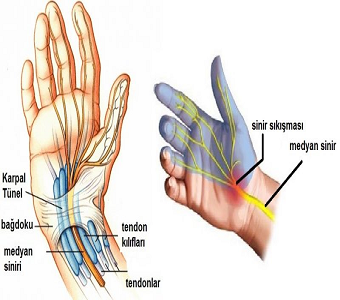
\includegraphics[width=4.72in]{figure/karpal_tunnel} 

}

\caption{Karpal Tünel Anatomisi ve Medyan Sinirin Sıkışması}\label{fig:unnamed-chunk-1}
\end{figure}
\hypertarget{KTSEpidemiyoloji}{%
\section{Epidemiyoloji}\label{KTSEpidemiyoloji}}

KTS prevalansı kadınlarda \%3 ila \%3.4 arasında, erkeklerde ise \%0.6 ila \% 2.7 arasında olarak
belirlenmiştir. İnsidans ise kadınlarda 100.000'de 140, erkeklerde 100.000'de 52 olarak saptanmıştır.
Kadınlarda genellikle menopoz dönemimde sıklıkla görülmüş olsa da hem erkek hem de kadınlarda
gözlenme sıklığı yaş ile doğru orantılıdır. Özellikle 20 ila 50 yaş arasında daha sıktır. KTS'nin \%40 ila \%60 oranında her iki elde de başlayabileceği çeşitli yayınlarda bildirilmiş olup, iki elde de görüldüğü olgularda baskın elin genellikle semptomları daha önce ve daha şiddetli gösterdiği söylenebilir. KTS tek elde görüldüğü durumlarda ise genellikle semptomlar baskın elde görülür (Bagatur, 2006).

\hypertarget{KTSEtiyoloji}{%
\section{Etiyoloji}\label{KTSEtiyoloji}}

Karpal tünel sendromunun en sık nedeni; herhangi bir etiyolojik etkenin saptanamadığı idiopatik KTS'dir. İdiopatik KTS'de ailesel yatkınlık, obezite, VKİ fazla olması, kara şeklinde bilek yapısı gibi
kişisel faktörlerin etken olduğu düşünülmektedir. Günlük yaşamda ki mekanik etkenler de idiopatik KTS
üzerinde etkin rol oynamaktadır. Montaj işinde çalışan işçiler, fabrika çalışanları, klavye ve bilgisayar
kullananlarda olduğu gibi el bilek fleksiyonun aktif olarak yapıldığı belli hareketlerin çok sık
tekrarlanması da KTS ile ilişkili bulunmuştur (Robbins, 1963).

\hypertarget{KTSSemptom}{%
\section{Semptomlar}\label{KTSSemptom}}

Hastalığın şiddetine bağlı olarak semptomlar değişkendir. Erken evrelerde medyan sinirin duyusal
liflerinin tutulumuna bağlı şikayetler görülür. En yaygın semptom el bileğinin merkezinden uzak
dokularda sızlama ve uyuşuklukla beraber yanıcı tarzda ağrıdır. Başparmak tarafından itibaren ilk üç
parmak ve dördüncü parmağın yanal yarısı etkilenir. Daha ileri dönemlerde el ayasında kas
güçsüzlüğü ve körelme meydana gelir . Bu hastalarda elde, özellikle aktivite ile artan beceriksizlik ve objeleri kavramada kuvvetsizlik görülür (Aroori ve Spence, 2008).

\hypertarget{KTSTani_Ciddi}{%
\section{Tanı ve Ciddiyet Değerlendirmesi}\label{KTSTani_Ciddi}}

Karpal tünel sendromunda tanı koymak için hastanın hikayesi, klinik semptomlar, fizik muayene bulguları ve bu bulguları destekleyen çeşitli testler kullanılmaktadır(Ghasemi-Rad ve diğerleri, 2014).
Bu testler elektronörofizyolojik, provokatif testler ve tıbbi görüntülemeye dayanan testlerdir.
Elektronörofizyolojik testler karpal Tünel'e bağlanan elektrotlar ile elektrik sinyallerinin incelenmesi ve sonuçların bilgisayar ile yorumlanmasına dayananan testlerdir.

\begin{figure}

{\centering 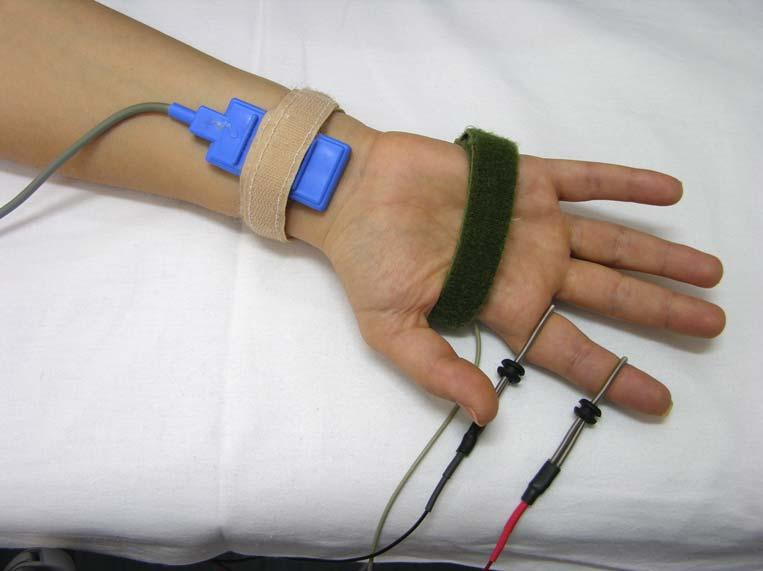
\includegraphics[width=0.49\linewidth,height=0.18\textheight]{figure/noropati_test} 

}

\caption{Elektronörofizyolojik Test (Kumaş, 2005)}\label{fig:unnamed-chunk-2}
\end{figure}
Provokatif testler hastanın bilek ve parmak eklemlerine fiziksel baskı uygulayacak şekilde bir takım
testler uygulanması ve alınan sonuçların değerlendirmesine dayanan deneysel test yöntemleridir.
Tanısal testler genellikle karpal tüneli görüntülemeye dayanan testlerdir.\\
* Phalen Testi\\
+ 60 saniye boyunca parmaklar ayak ucuna bakacak şekilde el dış yüzleri birleştirilir. Meydan sinir bölgesinde karıncalanma oluşur veya artarsa test pozitiftir.\\
* Ters Phalen testi\\
+ 60 saniye boyunca parmaklar yukarı bakacak şekilde el dış yüzleri birleştirilir. Meydan sinir bölgesinde karıncalanma oluşur veya artarsa test pozitiftir.\\
* Tinel testi\\
+ Uygulayıcı tarafından karpal tünelin üstüne perküsyon yapılır. Medyan sinir bölgesinde karıncalanma ve elektrik şoku hissi oluşursa test pozitiftir (Kurt, 2020).\\
* Karpal kompresyon testi\\
+ El bileği düz tutulurken medyan sinirin yakınına başparmak ile bastırılır. Medyan sinir bölgesinde karıncalanma oluşur veya artarsa test pozitiftir.\\
* Gerilmiş median sinir stres (GMSS) testi\\
+ Medyan sinir hareketliliğinin azaldığı durumlarda medyan sinirin gerilerek lokal iskeminin arttırılması mantığına dayanır.
\begin{figure}

{\centering 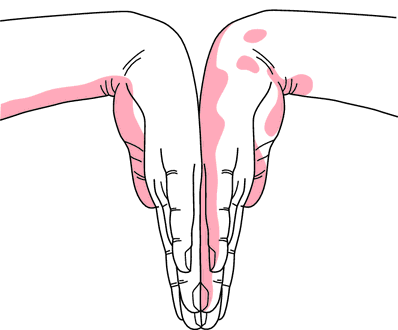
\includegraphics[width=0.49\linewidth,height=0.18\textheight]{figure/phalen} 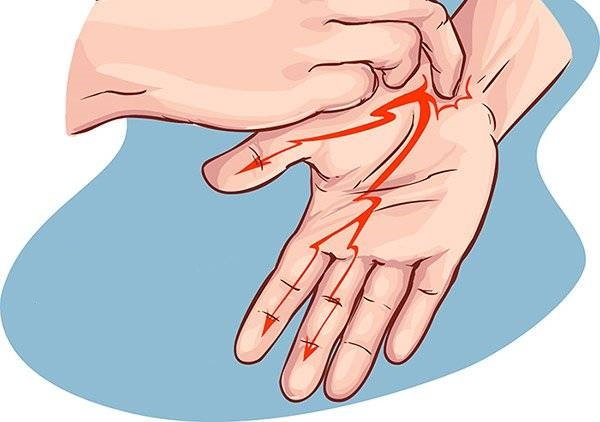
\includegraphics[width=0.49\linewidth,height=0.18\textheight]{figure/tinel} 

}

\caption{Phalen ve Tinel Testi}\label{fig:unnamed-chunk-3}
\end{figure}
\begin{figure}

{\centering 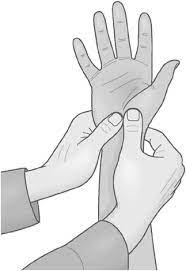
\includegraphics[width=0.49\linewidth,height=0.18\textheight]{figure/karpal_komp} 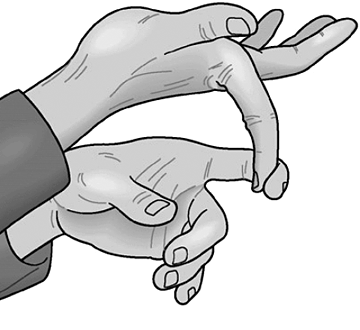
\includegraphics[width=0.49\linewidth,height=0.18\textheight]{figure/gerilmis} 

}

\caption{Karpal kompresyon ve GMSS Testi }\label{fig:unnamed-chunk-4}
\end{figure}
Görüntülemeye dayalı testlerde el bileği ve parmakların hareketi sırasında karpal tünel içerisindeki değişiklikleri ve medyan sinirin hareketlerini yorumlayarak hastaya tanı koymayı kolaylaştırır fakat hastalığın şiddeti hakkında bilgi vermez.\\
* Ultrasonografi\\
* Düz radyografi\\
* Bilgisayarlı tomografi\\
* Manyetik rezonans görüntüleme\\
\begin{figure}

{\centering 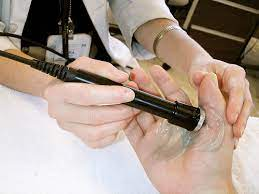
\includegraphics[width=0.49\linewidth,height=0.22\textheight]{figure/ultraradyo} 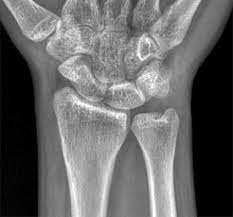
\includegraphics[width=0.49\linewidth,height=0.22\textheight]{figure/radyog} 

}

\caption{Ultrasonografi ve Düz radyografi }\label{fig:unnamed-chunk-5}
\end{figure}
\begin{figure}

{\centering 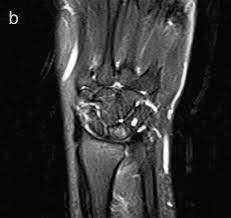
\includegraphics[width=0.49\linewidth,height=0.22\textheight]{figure/bt} 

}

\caption{Bilgisayarlı tomografi }\label{fig:unnamed-chunk-6}
\end{figure}
İdiopatik karpal tünel sendromunda hastalığın tanımlanmasında Boston Karpal Tünel Sendromu
Anketi(BKTSA) kullanılmaktadır (Levine ve diğerleri, 1993). Bu ankete farklı dillere çevrilmiş ve ülkelere göre uyarlanmıştır. Anketin amacı hastanın yanıtlarına göre bir ciddiyet sınıflandırması yapmaktır. Anketin Türkçe versiyonu Sezgin ve ark. (Sezgin ve diğerleri, 2006) tarafından yayımlanmıştır , ancak BKTSA sadece hastaların verdiği yanıtlara dayanarak bir semptom şiddeti belirlemeyi amaçlar.

Teknolojinin hızla gelişmesi ile birlikte hastalara uygulanan testlerin sonuçlarının toplanmasının kolaylaşmasının yanı sıra testlerin sonuçlarına bağlı olarak hastaya tanı koymak ve tanının şiddetini ve derecesini tespit etmek oldukça kolaylaşmıştır.\\
Makine öğrenmesi ve Yapay zeka uygulamalarının yaygınlaşması ile birlikte bu yöntemlerin tıp alanında da kullanımı artmıştır.

Makine öğrenmesi yöntemlerinin KTS tanısında kullanılmaına örnek olarak.
Ardakani ve ark. (Ardakani ve diğerleri, 2020) tarafından hasta olduğu bilinen kişilerden elde edilen bilgisayarlı tomografi görüntüleri, derin öğrenme metodları kullanılarak başka kişilerin hasta olup olmadığını tespit etmek için kullanılmıştır.\\
Bir diğer çalışma ise 2021 yılında Koyama ve ark. (Koyama ve diğerleri, 2021) tarafından geliştirilen bir mobil uygulama sayesinde hastaların ekranın farklı yerlerinde çıkan cisimlere ulaşma sürelerini baz alarak hastalığın evresini tahminlemeyi amaçlamıştır. Bu uygulama hastanın kendi kendine ev ortamında hastalığına ön tanı koyabilmesi açısından yararlı olabilir.\\
Bunların yanı sıra KTS ciddiyet skoru belirlemek için makine öğrenmesi yöntemlerini kullanan çalışmalar da yapılmaktadır.
Güncel bir çalışmada Park ve ark. (Park ve diğerleri, 2021) 1037 hastadan elde edilen verileri farklı makine öğrenmesi yöntemlerinde kullanarak KTS ciddiyet sınıflandırmasını tahmin etmeyi amaçlamışlardır.

\hypertarget{yontem}{%
\chapter{Yöntem}\label{yontem}}

Bu bölümde uygulama kısmında kullanmış olduğumuz sınıflama algoritmalarına değineceğiz.

\hypertarget{knn}{%
\section{K - En Yakın Komşuluk Algoritamsı (K-NN)}\label{knn}}

Öklid uzaklığı benzeri uzaklıklar ile tahminlenecek gözleme en yakın k adet gözlemin en fazla olduğu sınıfı atar.

\hypertarget{cart}{%
\section{Sınıflama ve Regresyon Ağaçları (CART)}\label{cart}}

İnsanın karar verme süreci olan dallanmış karar verme yapısını taklid eder.

\hypertarget{random_forest}{%
\section{Rassal Ormanlar}\label{random_forest}}

Torbalama yöntemi ile oluşturulmuş n adet karar ağacının sonuca göre çalışır.

\hypertarget{xgboost}{%
\section{Extreme Gradyan Artışı}\label{xgboost}}

NO COMMENT

\hypertarget{nn}{%
\section{Yapay Sinir Ağları}\label{nn}}

NO COMMENT

\hypertarget{deneme}{%
\section{DENEME}\label{deneme}}
\begin{itemize}
\tightlist
\item
  Liste1
\item
  Liste2
  \begin{itemize}
  \tightlist
  \item
    liste3
  \end{itemize}
\end{itemize}
\hypertarget{veri_seti}{%
\chapter{Veri Seti}\label{veri_seti}}

Veri setindeki düşük varyanslı değişken sayısı : 0
\begin{longtable}[]{@{}lr@{}}
\caption{\label{tab:deneme} Sayısal Değişkenlerin Tanımlayıcı İstatistikleri}\tabularnewline
\toprule
& Overall \\
\midrule
\endfirsthead
\toprule
& Overall \\
\midrule
\endhead
Age,years (mean \(\pm\) SD) & 58 \(\pm\) 10.8 \\
BMI, kg/m\(^2\) (mean \(\pm\) SD) & 24.8 \(\pm\) 3.4 \\
Duration, months (mean \(\pm\) SD) & 8.3 \(\pm\) 9.6 \\
NRS (mean \(\pm\) SD) & 4.4 \(\pm\) 1.8 \\
CSA, mm\(^2\) (mean \(\pm\) SD) & 15.2 \(\pm\) 4.3 \\
PB, mm (mean \(\pm\) SD) & 2.5 \(\pm\) 1.8 \\
\bottomrule
\end{longtable}
\begin{longtable}[]{@{}lrrrr@{}}
\caption{\label{tab:descrip} Değişkenlerin Bağımlı Değişkene Göre Tanımlayıcı İstatistikleri \tiny (P-Value Değerleri Tek Yönlü Varyans Analiz Testi ile Elde Edilmiştir.)}\tabularnewline
\toprule
& Mild & Moderate & Severe & P Value \\
\midrule
\endfirsthead
\toprule
& Mild & Moderate & Severe & P Value \\
\midrule
\endhead
Age,years (mean \(\pm\) SD) & 57.3 \(\pm\) 10.6 & 59.2 \(\pm\) 10.8 & 57.8 \(\pm\) 11.2 & 0.069 \\
BMI, kg/m\(^2\) (mean \(\pm\) SD) & 24.2 \(\pm\) 3.4 & 24.7 \(\pm\) 3 & 25.8 \(\pm\) 3.7 & 0 \\
Duration, months (mean \(\pm\) SD) & 4.3 \(\pm\) 5 & 8.5 \(\pm\) 8.2 & 15.9 \(\pm\) 12.8 & 0 \\
NRS (mean \(\pm\) SD) & 3.3 \(\pm\) 1.3 & 4.9 \(\pm\) 1.5 & 6.1 \(\pm\) 1.5 & 0 \\
CSA, mm\(^2\) (mean \(\pm\) SD) & 13.2 \(\pm\) 3 & 15.4 \(\pm\) 3.2 & 18.9 \(\pm\) 5 & 0 \\
PB, mm (mean \(\pm\) SD) & 2.1 \(\pm\) 0.8 & 2.6 \(\pm\) 2.4 & 3.1 \(\pm\) 2.3 & 0 \\
\bottomrule
\end{longtable}
\hfill\break
\hfill\break
~
\begin{longtable}[]{@{}lrrrr@{}}
\caption{\label{tab:catvar} Katagorik Değişkenlerin Bağımlı Değişkence Frekans Dağılımı \tiny (P-Value Değerleri Ki-Kare Bağımsızlık Testi ile Elde Edilmiştir.)}\tabularnewline
\toprule
& Mild & Moderate & Severe & P value \\
\midrule
\endfirsthead
\toprule
& Mild & Moderate & Severe & P value \\
\midrule
\endhead
Eller, n (\%) & 507 (48.9) & 276 (26.6) & 254 (24.5) & - \\
Cinsiyet (Kadın), n (\%) & 308 (60.7) & 153 (55.4) & 171 (67.3) & 0.02 \\
Sağ El Kasılması, n (\%) & 243 (47.9) & 149 (54) & 119 (46.9) & 0.181 \\
Diyabet, n (\%) & 47 (9.3) & 45 (16.3) & 54 (21.3) & 0 \\
Gece Ağrıları, n (\%) & 102 (20.1) & 142 (51.4) & 212 (83.5) & 0 \\
Avuç İçi Zayıflık ve/veya Körelme, n (\%) & 1 (0.2) & 24 (8.7) & 169 (66.5) & 0 \\
\bottomrule
\end{longtable}
\hypertarget{k-en-yakux131n-komux15fuluk-modeli}{%
\section{K-En Yakın Komşuluk Modeli}\label{k-en-yakux131n-komux15fuluk-modeli}}

Bu bölümde veri setimiz üzerinde K - En yakın komşuluk modelini kullanacak ve çıktılarını değerlendireceğiz.

\hypertarget{hiper-parametre-seuxe7imi}{%
\subsection{Hiper Parametre Seçimi}\label{hiper-parametre-seuxe7imi}}

Daha önce belirlediğimiz parametre uzayını ve Scikit-Learn kütüphanesinde bulunan GridSearchCV algoritması ile en uygun doğruluk oranını yakalayana kadar çalışması sağlandı.
\begin{figure}

{\centering 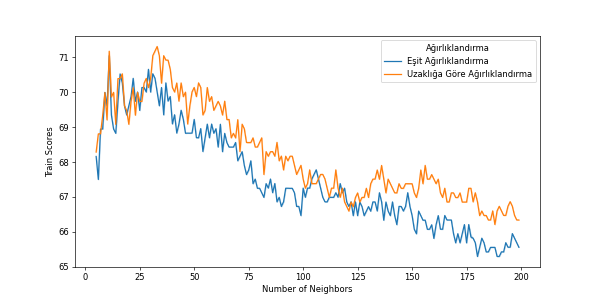
\includegraphics[width=1.1\linewidth,height=0.55\textheight]{figure/KNN_Grid_Graph} 

}

\caption{Model Train Scores}\label{fig:unnamed-chunk-13}
\end{figure}
\begin{verbatim}
En İyi Parametreler:{'algorithm':'auto','n_neighbors':33,'weights':'distance'}
\end{verbatim}
\hypertarget{en-iyi-parametreli-model}{%
\subsection{En İyi Parametreli Model}\label{en-iyi-parametreli-model}}

GridSearchCV algoritması ile bulduğumuz parametrelerle kurulan modelimizin sınıflandırma metrikleri.
\begin{verbatim}
              precision    recall  f1-score   support

        Mild       0.76      0.92      0.83       137
    Moderate       0.51      0.42      0.46        65
      Severe       0.89      0.68      0.77        72

    accuracy                           0.74       274
   macro avg       0.72      0.67      0.69       274
weighted avg       0.73      0.74      0.73       274
\end{verbatim}
\begin{verbatim}
Balanced Accuracy Score : 0.6718827333790838
\end{verbatim}
\begin{figure}

{\centering 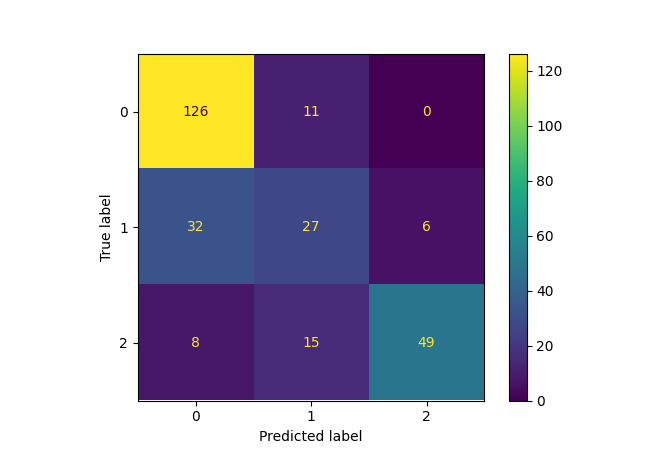
\includegraphics[width=1.05\linewidth,height=0.6\textheight]{figure/knn_conf} 

}

\caption{K-En Yakın Komşuluk Modeli Karmaşıklık Matrisi}\label{fig:unnamed-chunk-18}
\end{figure}
\begin{figure}

{\centering 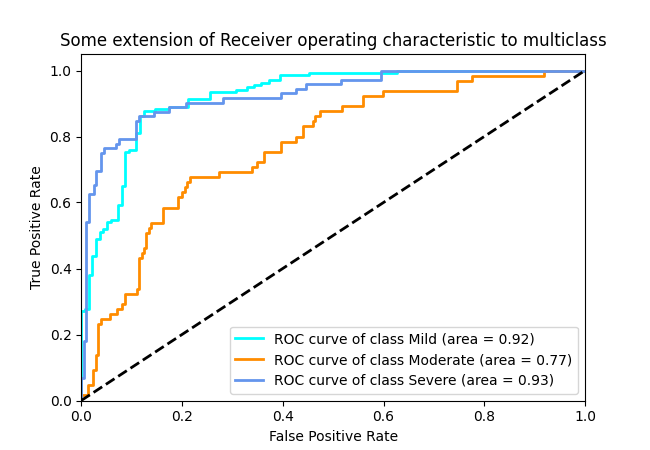
\includegraphics[width=1.05\linewidth,height=0.6\textheight]{figure/roc_curve_KNeighborsClassifier} 

}

\caption{K-En Yakın Komşuluk Modeli ROC Eğrisi ve AUC Değeri}\label{fig:unnamed-chunk-19}
\end{figure}
\hypertarget{rassal-ormanlar-modeli}{%
\section{Rassal Ormanlar Modeli}\label{rassal-ormanlar-modeli}}

Bu bölümde veri setimiz üzerinde Rassal Ormanlar modelini kullanacak ve çıktılarını değerlendireceğiz.

\hypertarget{hiper-parametre-seuxe7imi-1}{%
\subsection{Hiper Parametre Seçimi}\label{hiper-parametre-seuxe7imi-1}}

Daha önce belirlediğimiz parametre uzayını ve Scikit-Learn kütüphanesinde bulunan GridSearchCV algoritması ile en uygun doğruluk oranını yakalayana kadar çalışması sağlandı.
\begin{figure}

{\centering 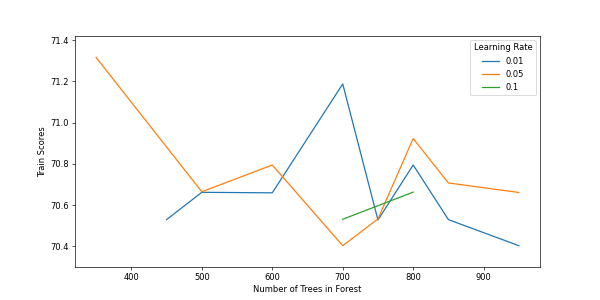
\includegraphics[width=1.1\linewidth,height=0.5\textheight]{figure/RF_Grid_Graph} 

}

\caption{Model Train Scores}\label{fig:unnamed-chunk-21}
\end{figure}
\begin{verbatim}
En İyi Parametreler:{'ccp_alpha':0.05,'criterion':'gini','max_features':'auto',
'max_samples':10,'n_estimators':350}
\end{verbatim}
\hypertarget{en-iyi-parametreli-model-1}{%
\subsection{En İyi Parametreli Model}\label{en-iyi-parametreli-model-1}}

GridSearchCV algoritması ile bulduğumuz parametrelerle kurulan modelimizin sınıflandırma metrikleri.
\begin{verbatim}
              precision    recall  f1-score   support

        Mild       0.73      0.99      0.84       137
    Moderate       0.58      0.34      0.43        65
      Severe       0.94      0.68      0.79        72

    accuracy                           0.75       274
   macro avg       0.75      0.67      0.69       274
weighted avg       0.75      0.75      0.73       274
\end{verbatim}
\begin{verbatim}
Balanced Accuracy Score : 0.6681395179570361
\end{verbatim}
\begin{figure}

{\centering 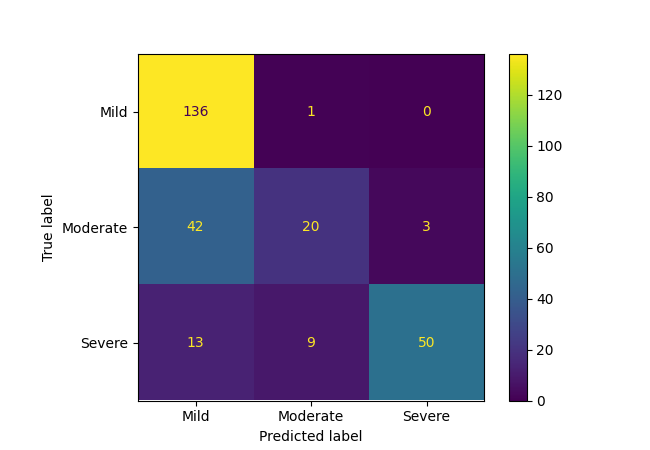
\includegraphics[width=1.05\linewidth,height=0.6\textheight]{figure/rfc_conf} 

}

\caption{Rassal Ormanlar Modeli Karmaşıklık Matrisi}\label{fig:unnamed-chunk-26}
\end{figure}
\begin{figure}

{\centering 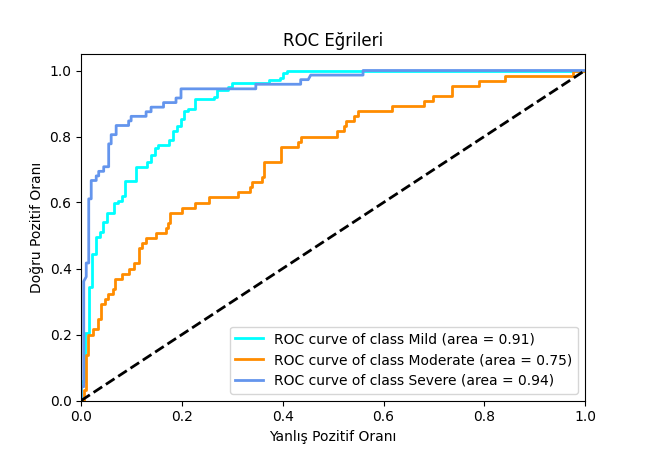
\includegraphics[width=1.05\linewidth,height=0.6\textheight]{figure/roc_curve_RandomForestClassifier} 

}

\caption{Rassal Ormanlar Modeli ROC Eğrisi ve AUC Değeri}\label{fig:unnamed-chunk-27}
\end{figure}
\hypertarget{extreme-gradient-boosting-xgboost}{%
\section{eXtreme Gradient Boosting (Xgboost)}\label{extreme-gradient-boosting-xgboost}}

\hypertarget{Bolum4}{%
\chapter{Bölüm 4 Başlık}\label{Bolum4}}

\hypertarget{bu-bir-alt-baux15flux131k}{%
\section{Bu bir alt başlık}\label{bu-bir-alt-baux15flux131k}}

Bu bölümde şu konular yer almaktadır\ldots{}

\hypertarget{bu-ikinci-seviye-bir-alt-baux15flux131k}{%
\subsection{Bu ikinci seviye bir alt başlık}\label{bu-ikinci-seviye-bir-alt-baux15flux131k}}

\hypertarget{sonuuxe7}{%
\chapter*{Sonuç}\label{sonuuxe7}}
\addcontentsline{toc}{chapter}{Sonuç}

If we don't want Conclusion to have a chapter number next to it, we can add the \texttt{\{-\}} attribute.

\textbf{More info}

And here's some other random info: the first paragraph after a chapter title or section head \emph{shouldn't be} indented, because indents are to tell the reader that you're starting a new paragraph. Since that's obvious after a chapter or section title, proper typesetting doesn't add an indent there.

\hypertarget{kaynaklar}{%
\chapter*{Kaynaklar}\label{kaynaklar}}
\addcontentsline{toc}{chapter}{Kaynaklar}

\markboth{Kaynaklar}{Kaynaklar}

\hypertarget{refs}{}
\begin{CSLReferences}{1}{0}
\leavevmode\vadjust pre{\hypertarget{ref-ardakani2020diagnosis}{}}%
Ardakani, A. A., Afshar, A., Bhatt, S., Bureau, N. J., Tahmasebi, A., Acharya, U. R. ve Mohammadi, A. (2020). Diagnosis of carpal tunnel syndrome: A comparative study of shear wave elastography, morphometry and artificial intelligence techniques. \emph{Pattern Recognition Letters}, \emph{133}, 77-85.

\leavevmode\vadjust pre{\hypertarget{ref-aroori77carpal}{}}%
Aroori, S. ve Spence, R. (2008). Carpal Tunnel Syndrome. \emph{The Ulster Medical Society}, \emph{77}, 1-17.

\leavevmode\vadjust pre{\hypertarget{ref-kts_bagatur}{}}%
Bagatur, A. E. (2006). Karpal Tünel Sendromu. \emph{Türkiye Klinikleri J Surg Med Sci.}, \emph{2}(17), 52-63.

\leavevmode\vadjust pre{\hypertarget{ref-ghasemi2014handy}{}}%
Ghasemi-Rad, M., Nosair, E., Vegh, A., Mohammadi, A., Akkad, A., Lesha, E., \ldots{} others. (2014). A handy review of carpal tunnel syndrome: From anatomy to diagnosis and treatment. \emph{World journal of radiology}, \emph{6}(6), 284.

\leavevmode\vadjust pre{\hypertarget{ref-koyama2021screening}{}}%
Koyama, T., Sato, S., Toriumi, M., Watanabe, T., Nimura, A., Okawa, A., \ldots{} Fujita, K. (2021). A Screening Method Using Anomaly Detection on a Smartphone for Patients With Carpal Tunnel Syndrome: Diagnostic Case-Control Study. \emph{JMIR mHealth and uHealth}, \emph{9}(3), e26320.

\leavevmode\vadjust pre{\hypertarget{ref-kumacs2005idiyopatik}{}}%
Kumaş, F. F. (2005).{I}diyopatik karpal t{"u}nel sendromu tedavisinde terap{"o}tik ultrason, steroid enjeksiyonu ve splint kullan{ı}m{ı}n{ı}n etkinli{ğ}inin randimize kontroll{"u} ara{ş}t{ı}r{ı}lmas{ı}.

\leavevmode\vadjust pre{\hypertarget{ref-kurt2020karpal}{}}%
Kurt, A. (2020). \emph{Karpal t{"u}nel sendrom hastalar{ı}nda bilateral ince motor beceri, skapular diskinezi, hareket korkusu ve fonksiyonun sa{ğ}l{ı}kl{ı}larla kar{ş}{ı}la{ş}t{ı}r{ı}lmas{ı}}. (Yayımlanmamış mathesis). Sa{ğ}l{ı}k Bilimleri Enstit{"u}s{"u}.

\leavevmode\vadjust pre{\hypertarget{ref-levine1993self}{}}%
Levine, D. W., Simmons, B. P., Koris, M. J., Daltroy, L. H., Hohl, G. G., Fossel, A. H. ve Katz, J. N. (1993). A self-administered questionnaire for the assessment of severity of symptoms and functional status in carpal tunnel syndrome. \emph{The Journal of bone and joint surgery. American volume}, \emph{75}(11), 1585-1592.

\leavevmode\vadjust pre{\hypertarget{ref-1995love}{}}%
Love, J. (1955). Median neuritis or carpal tunnel syndrome; diagnosis and treatment. \emph{North Carolina medical journal}, \emph{16}(10), 463-469.

\leavevmode\vadjust pre{\hypertarget{ref-park2021machine}{}}%
Park, D., Kim, B. H., Lee, S.-E., Kim, D. Y., Kim, M., Kwon, H. D., \ldots{} Lee, J. W. (2021). Machine learning-based approach for disease severity classification of carpal tunnel syndrome. \emph{Scientific Reports}, \emph{11}(1), 1-10.

\leavevmode\vadjust pre{\hypertarget{ref-history1988}{}}%
Pfeffer, G., Gelberman, R., Boyes, J. ve Rydevik, B. (1988). The history of carpal tunnnel syndrome. \emph{The Journal of Hand Surgery: British \& European Volume}, \emph{13}(1), 28-34.

\leavevmode\vadjust pre{\hypertarget{ref-robbins1963anatomical}{}}%
Robbins, H. (1963). Anatomical study of the median nerve in the carpal tunnel and etiologies of the carpal-tunnel syndrome. \emph{JBJS}, \emph{45}(5), 953-966.

\leavevmode\vadjust pre{\hypertarget{ref-sezgi2006assessment}{}}%
Sezgin, M.,.Incel, N. A., Sevi˙ m, S., ren, H. Çamdevi˙, As, I. ve ErdoĞan, C. (2006). Assessment of symptom severity and functional status in patients with carpal tunnel syndrome: reliability and validity of the Turkish version of the Boston Questionnaire. \emph{Disability and rehabilitation}, \emph{28}(20), 1281-1286.

\leavevmode\vadjust pre{\hypertarget{ref-werner2002carpal}{}}%
Werner, R. A. ve Andary, M. (2002). Carpal tunnel syndrome: pathophysiology and clinical neurophysiology. \emph{Clinical Neurophysiology}, \emph{113}(9), 1373-1381.

\end{CSLReferences}
\setlength{\parindent}{-0.20in}
\setlength{\leftskip}{0.20in}
\setlength{\parskip}{8pt}

\appendix

\hypertarget{ilk-ek-baux15flux131ux11fux131}{%
\chapter{İlk Ek Başlığı}\label{ilk-ek-baux15flux131ux11fux131}}

This first appendix includes all of the R chunks of code that were hidden throughout the document (using the \texttt{include\ =\ FALSE} chunk tag) to help with readibility and/or setup.

\textbf{In the main Rmd file}
\begin{Shaded}
\begin{Highlighting}[]
\CommentTok{\# This chunk ensures that the thesisdown package is}
\CommentTok{\# installed and loaded. This thesisdown package includes}
\CommentTok{\# the template files for the thesis.}
 \ControlFlowTok{if}\NormalTok{(}\SpecialCharTok{!}\FunctionTok{require}\NormalTok{(remotes)) }\FunctionTok{install.packages}\NormalTok{(}\StringTok{"remotes"}\NormalTok{, }\AttributeTok{repos =} \StringTok{"http://cran.rstudio.com"}\NormalTok{)}
 \ControlFlowTok{if}\NormalTok{(}\SpecialCharTok{!}\FunctionTok{require}\NormalTok{(thesisdown))remotes}\SpecialCharTok{::}\FunctionTok{install\_github}\NormalTok{(}\StringTok{"ismayc/thesisdown"}\NormalTok{)}
 \FunctionTok{library}\NormalTok{(thesisdown)}
\end{Highlighting}
\end{Shaded}
\textbf{In Chapter \ref{ref-labels}:}

\hypertarget{ikinci-ek-baux15flux131ux11fux131}{%
\chapter{İkinci Ek Başlığı}\label{ikinci-ek-baux15flux131ux11fux131}}

İkinci Ek




\end{document}
